\documentclass[11pt, a4paper]{article}\usepackage[]{graphicx}\usepackage[]{xcolor}
% maxwidth is the original width if it is less than linewidth
% otherwise use linewidth (to make sure the graphics do not exceed the margin)
\makeatletter
\def\maxwidth{ %
  \ifdim\Gin@nat@width>\linewidth
    \linewidth
  \else
    \Gin@nat@width
  \fi
}
\makeatother

\definecolor{fgcolor}{rgb}{0.345, 0.345, 0.345}
\newcommand{\hlnum}[1]{\textcolor[rgb]{0.686,0.059,0.569}{#1}}%
\newcommand{\hlsng}[1]{\textcolor[rgb]{0.192,0.494,0.8}{#1}}%
\newcommand{\hlcom}[1]{\textcolor[rgb]{0.678,0.584,0.686}{\textit{#1}}}%
\newcommand{\hlopt}[1]{\textcolor[rgb]{0,0,0}{#1}}%
\newcommand{\hldef}[1]{\textcolor[rgb]{0.345,0.345,0.345}{#1}}%
\newcommand{\hlkwa}[1]{\textcolor[rgb]{0.161,0.373,0.58}{\textbf{#1}}}%
\newcommand{\hlkwb}[1]{\textcolor[rgb]{0.69,0.353,0.396}{#1}}%
\newcommand{\hlkwc}[1]{\textcolor[rgb]{0.333,0.667,0.333}{#1}}%
\newcommand{\hlkwd}[1]{\textcolor[rgb]{0.737,0.353,0.396}{\textbf{#1}}}%
\let\hlipl\hlkwb

\usepackage{framed}
\makeatletter
\newenvironment{kframe}{%
 \def\at@end@of@kframe{}%
 \ifinner\ifhmode%
  \def\at@end@of@kframe{\end{minipage}}%
  \begin{minipage}{\columnwidth}%
 \fi\fi%
 \def\FrameCommand##1{\hskip\@totalleftmargin \hskip-\fboxsep
 \colorbox{shadecolor}{##1}\hskip-\fboxsep
     % There is no \\@totalrightmargin, so:
     \hskip-\linewidth \hskip-\@totalleftmargin \hskip\columnwidth}%
 \MakeFramed {\advance\hsize-\width
   \@totalleftmargin\z@ \linewidth\hsize
   \@setminipage}}%
 {\par\unskip\endMakeFramed%
 \at@end@of@kframe}
\makeatother

\definecolor{shadecolor}{rgb}{.97, .97, .97}
\definecolor{messagecolor}{rgb}{0, 0, 0}
\definecolor{warningcolor}{rgb}{1, 0, 1}
\definecolor{errorcolor}{rgb}{1, 0, 0}
\newenvironment{knitrout}{}{} % an empty environment to be redefined in TeX

\usepackage{alltt}

\usepackage[top=1 in, bottom = 1 in, left = 1 in, right = 1 in ]{geometry}

\usepackage{amsmath, amssymb, amsfonts}
\usepackage{enumerate}
\usepackage{array}
\usepackage{multirow}
\usepackage{dingbat}
\usepackage{fontawesome5}
\usepackage{tasks}

\title{MSMS - 106}
\author{Ananda Biswas}
\date{}
\IfFileExists{upquote.sty}{\usepackage{upquote}}{}
\begin{document}

\maketitle

\begin{center}
\textbf{Practical 05}
\end{center}


\smallpencil \hspace{0.5cm} Fit a poisson distribution to the given data-set.

\begin{table}[!htbp]
\def\arraystretch{1.5}

\begin{center}
\begin{tabular}{|>{\centering}m{1cm}||>{\centering}m{1cm}|>{\centering}m{1cm}|>{\centering}m{1cm}|>{\centering}m{1cm}|>{\centering}m{1cm}|>{\centering}m{1cm}|>{\centering}m{1cm}|>{\centering}m{1cm}|>{\centering}m{1cm}|>{\centering\arraybackslash}m{2cm}|}

\hline

$x$ & 0 & 1 & 2 & 3 & 4 & 5 & 6 & 7 & 8 & 9 or more \\

\hline

$f$ & 162 & 193 & 115 & 83 & 44 & 24 & 19 & 8 & 2 & 0 \\

\hline

\end{tabular}
\end{center}
\end{table}

Also perform a $\chi^2$ goodness of fit test. \\

\faArrowAltCircleRight[regular] \textit{\textbf{Fitting a Poisson Distribution}} \\

The P.M.F. of a Poisson distribution is $P(X = x) = e^{-\lambda} \cdot \dfrac{\lambda^x}{x!} \,\, ; x = 0, 1, 2, 3, \ldots \,\, ,\lambda > 0$. \\

We estimate parameter $\lambda$ as $\hat{\lambda} = \bar{x} = \dfrac{\sum \limits_{i = 0}^{\infty} x_i f_i}{\sum \limits_{i = 0}^{\infty} f_i}$.


\begin{knitrout}
\definecolor{shadecolor}{rgb}{0.969, 0.969, 0.969}\color{fgcolor}\begin{kframe}
\begin{alltt}
\hldef{x} \hlkwb{<-} \hlnum{0}\hlopt{:}\hlnum{9}
\hldef{freq} \hlkwb{<-} \hlkwd{c}\hldef{(}\hlnum{162}\hldef{,} \hlnum{193}\hldef{,} \hlnum{115}\hldef{,} \hlnum{83}\hldef{,} \hlnum{44}\hldef{,} \hlnum{24}\hldef{,} \hlnum{19}\hldef{,} \hlnum{8}\hldef{,} \hlnum{2}\hldef{,} \hlnum{0}\hldef{)}
\end{alltt}
\end{kframe}
\end{knitrout}

\begin{knitrout}
\definecolor{shadecolor}{rgb}{0.969, 0.969, 0.969}\color{fgcolor}\begin{kframe}
\begin{alltt}
\hldef{weighted_mean} \hlkwb{<-} \hlkwa{function}\hldef{(}\hlkwc{x}\hldef{,} \hlkwc{weight}\hldef{)\{}
  \hldef{xw} \hlkwb{<-} \hlnum{0}
  \hldef{w} \hlkwb{<-} \hlnum{0}
  \hlkwa{for} \hldef{(i} \hlkwa{in} \hlnum{1}\hlopt{:}\hlkwd{length}\hldef{(x)) \{}
    \hldef{xw} \hlkwb{<-} \hldef{xw} \hlopt{+} \hldef{x[i]} \hlopt{*} \hldef{weight[i]}
    \hldef{w} \hlkwb{<-} \hldef{w} \hlopt{+} \hldef{weight[i]}
  \hldef{\}}
  \hlkwd{return}\hldef{(xw} \hlopt{/} \hldef{w)}
\hldef{\}}
\end{alltt}
\end{kframe}
\end{knitrout}

\begin{knitrout}
\definecolor{shadecolor}{rgb}{0.969, 0.969, 0.969}\color{fgcolor}\begin{kframe}
\begin{alltt}
\hldef{x_bar} \hlkwb{<-} \hlkwd{weighted_mean}\hldef{(x, freq)}
\hldef{x_bar}
\end{alltt}
\begin{verbatim}
## [1] 1.775385
\end{verbatim}
\end{kframe}
\end{knitrout}

$\bar{x}$ = 1.7753846. So $\hat{\lambda}$ = 1.7753846. Now we fit $Poisson$(1.7753846) distribution to the given data. \\

Now $P(X = 0) = e^{-1.7753846}$ = 0.1694183 and \\

$P(X = i + 1) = \dfrac{\lambda}{i + 1} \cdot P(X = i); \,\, i = 0,1,2,\ldots .$ \\

Also, expected frequency of $i = k \cdot P(X = i); \,\, i = 0,1,2,\ldots$, where $k = \sum \limits_{i = 0}^{\infty} f_i$ is the total frequency.

\begin{knitrout}\footnotesize
\definecolor{shadecolor}{rgb}{0.969, 0.969, 0.969}\color{fgcolor}\begin{kframe}
\begin{alltt}
\hldef{lambda} \hlkwb{<-} \hldef{x_bar}
\end{alltt}
\end{kframe}
\end{knitrout}

\begin{knitrout}\footnotesize
\definecolor{shadecolor}{rgb}{0.969, 0.969, 0.969}\color{fgcolor}\begin{kframe}
\begin{alltt}
\hldef{probabilities} \hlkwb{<-} \hlkwd{c}\hldef{(}\hlkwd{exp}\hldef{(}\hlopt{-}\hldef{lambda))}

\hldef{i} \hlkwb{<-} \hlnum{1}
\hlkwa{while} \hldef{(i} \hlopt{<=} \hlnum{8}\hldef{) \{}
  \hldef{probabilities[i}\hlopt{+}\hlnum{1}\hldef{]} \hlkwb{<-} \hldef{(lambda} \hlopt{/} \hldef{x[i}\hlopt{+}\hlnum{1}\hldef{])} \hlopt{*} \hldef{probabilities[i]}

  \hldef{i} \hlkwb{<-} \hldef{i} \hlopt{+} \hlnum{1}
\hldef{\}}
\end{alltt}
\end{kframe}
\end{knitrout}

\begin{knitrout}\footnotesize
\definecolor{shadecolor}{rgb}{0.969, 0.969, 0.969}\color{fgcolor}\begin{kframe}
\begin{alltt}
\hldef{total_frequency} \hlkwb{<-} \hlnum{0}

\hlkwa{for} \hldef{(i} \hlkwa{in} \hlnum{1}\hlopt{:}\hlkwd{length}\hldef{(freq)) \{}
  \hldef{total_frequency} \hlkwb{<-} \hldef{total_frequency} \hlopt{+} \hldef{freq[i]}
\hldef{\}}
\end{alltt}
\end{kframe}
\end{knitrout}

\begin{knitrout}\footnotesize
\definecolor{shadecolor}{rgb}{0.969, 0.969, 0.969}\color{fgcolor}\begin{kframe}
\begin{alltt}
\hldef{expected_frequencies} \hlkwb{<-} \hlkwd{c}\hldef{()}

\hlkwa{for} \hldef{(i} \hlkwa{in} \hlnum{1}\hlopt{:}\hlnum{9}\hldef{) \{}
  \hldef{expected_frequencies[i]} \hlkwb{<-} \hldef{probabilities[i]} \hlopt{*} \hldef{total_frequency}
\hldef{\}}
\end{alltt}
\end{kframe}
\end{knitrout}

And $P(X \geq 9) = 1 - P(X \leq 8)$ = \ensuremath{9.9084863\times 10^{-5}}. \\

Here is our fit.

\begin{knitrout}\footnotesize
\definecolor{shadecolor}{rgb}{0.969, 0.969, 0.969}\color{fgcolor}\begin{kframe}
\begin{alltt}
\hldef{df} \hlkwb{<-} \hlkwd{data.frame}\hldef{(}\hlkwc{x} \hldef{=} \hlkwd{c}\hldef{(}\hlnum{0}\hlopt{:}\hlnum{8}\hldef{,} \hlsng{"9 or more"}\hldef{),}
                 \hlkwc{observed} \hldef{= freq,}
                 \hlkwc{expected} \hldef{=} \hlkwd{c}\hldef{(expected_frequencies,}
                              \hldef{total_frequency} \hlopt{*} \hldef{(}\hlnum{1} \hlopt{-} \hlkwd{sum}\hldef{(probabilities))))}
\hldef{df}
\end{alltt}
\begin{verbatim}
##            x observed     expected
## 1          0      162 110.12187946
## 2          1      193 195.50869061
## 3          2      115 173.55156074
## 4          3       83 102.70692364
## 5          4       44  45.58607303
## 6          5       24  16.18656255
## 7          6       19   4.78956235
## 8          7        8   1.21475933
## 9          8        2   0.26958313
## 10 9 or more        0   0.06440516
\end{verbatim}
\end{kframe}
\end{knitrout}

\begin{knitrout}
\definecolor{shadecolor}{rgb}{0.969, 0.969, 0.969}\color{fgcolor}\begin{kframe}
\begin{alltt}
\hlkwd{sum}\hldef{(df}\hlopt{$}\hldef{observed);} \hlkwd{sum}\hldef{(df}\hlopt{$}\hldef{expected)}
\end{alltt}
\begin{verbatim}
## [1] 650
## [1] 650
\end{verbatim}
\end{kframe}
\end{knitrout}

Total expected frequency and total observed frequency are also equal.

\newpage

A visualization of the fit will be great.

\begin{knitrout}
\definecolor{shadecolor}{rgb}{0.969, 0.969, 0.969}\color{fgcolor}\begin{kframe}
\begin{alltt}
\hlkwd{library}\hldef{(tidyverse)}
\end{alltt}
\end{kframe}
\end{knitrout}

\begin{knitrout}
\definecolor{shadecolor}{rgb}{0.969, 0.969, 0.969}\color{fgcolor}\begin{kframe}
\begin{alltt}
\hldef{df_melted} \hlkwb{<-} \hldef{df} \hlopt
                \hlkwd{pivot_longer}\hldef{(}\hlkwc{cols} \hldef{=} \hlkwd{c}\hldef{(}\hlsng{"observed"}\hldef{,} \hlsng{"expected"}\hldef{),}
                             \hlkwc{names_to} \hldef{=} \hlsng{"frequency_type"}\hldef{,}
                             \hlkwc{values_to} \hldef{=} \hlsng{"frequency"}\hldef{)}
\end{alltt}
\end{kframe}
\end{knitrout}

\begin{knitrout}
\definecolor{shadecolor}{rgb}{0.969, 0.969, 0.969}\color{fgcolor}\begin{kframe}
\begin{alltt}
\hldef{df_melted} \hlopt
  \hlkwd{ggplot}\hldef{(}\hlkwd{aes}\hldef{(}\hlkwc{x} \hldef{= x,} \hlkwc{y} \hldef{= frequency,} \hlkwc{fill} \hldef{= frequency_type))} \hlopt{+}
  \hlkwd{geom_col}\hldef{(}\hlkwc{position} \hldef{=} \hlsng{"dodge"}\hldef{)} \hlopt{+}
  \hlkwd{labs}\hldef{(}\hlkwc{x} \hldef{=} \hlsng{"x"}\hldef{,} \hlkwc{title} \hldef{=} \hlsng{"Visualizing the fit"}\hldef{)} \hlopt{+}
  \hlkwd{theme}\hldef{(}\hlkwc{legend.position} \hldef{=} \hlsng{"top"}\hldef{)}
\end{alltt}
\end{kframe}
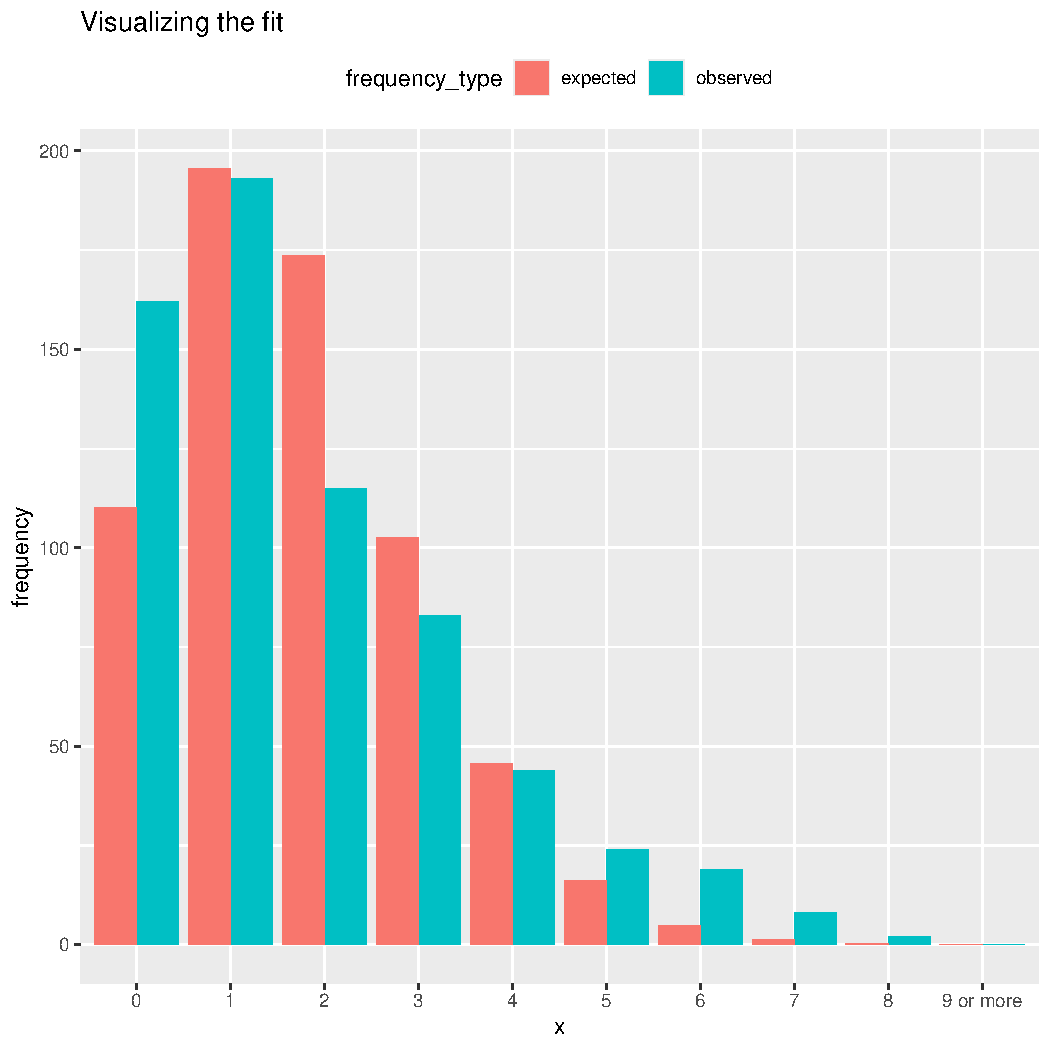
\includegraphics[width=\maxwidth]{figure/unnamed-chunk-12-1} 
\end{knitrout}

\newpage

\faArrowAltCircleRight[regular] \textit{\textbf{$\chi^2$ Goodness of fit test}} \\

$\chi^2 = \sum \limits_{i = 1}^{m} \dfrac{(f_i - kp_i)^2}{kp_i}$ where $m$ is the number of classes, $f_i$ is the observed frequency of $i$-th class, \\

$p_i$ is the theoretical probability of belonging to $i$-th class, $k$ is total frequency. \\

In large sample, $\chi^2 \sim \chi^2_{m-1-u}$, where $u$ is the number of parameters estimated from the data. \\

We also must have expected frequency greater than or equal to 5 for each class. \\

Here, in order to achieve so, we shall combine last 4 classes.

\begin{knitrout}
\definecolor{shadecolor}{rgb}{0.969, 0.969, 0.969}\color{fgcolor}\begin{kframe}
\begin{alltt}
\hldef{new_df} \hlkwb{<-} \hlkwd{data.frame}\hldef{(}\hlkwc{x} \hldef{=} \hlkwd{c}\hldef{(}\hlnum{0}\hlopt{:}\hlnum{5}\hldef{,} \hlsng{"6 or more"}\hldef{),}
                     \hlkwc{observed} \hldef{=} \hlkwd{c}\hldef{(df[}\hlnum{1}\hlopt{:}\hlnum{6}\hldef{,} \hlnum{2}\hldef{],} \hlkwd{sum}\hldef{(df[}\hlnum{7}\hlopt{:}\hlnum{10}\hldef{,} \hlnum{2}\hldef{])),}
                     \hlkwc{expected} \hldef{=} \hlkwd{c}\hldef{(df[}\hlnum{1}\hlopt{:}\hlnum{6}\hldef{,} \hlnum{3}\hldef{],} \hlkwd{sum}\hldef{(df[}\hlnum{7}\hlopt{:}\hlnum{10}\hldef{,} \hlnum{3}\hldef{])))}
\end{alltt}
\end{kframe}
\end{knitrout}

Now we have

\begin{knitrout}
\definecolor{shadecolor}{rgb}{0.969, 0.969, 0.969}\color{fgcolor}\begin{kframe}
\begin{alltt}
\hldef{new_df}
\end{alltt}
\begin{verbatim}
##           x observed  expected
## 1         0      162 110.12188
## 2         1      193 195.50869
## 3         2      115 173.55156
## 4         3       83 102.70692
## 5         4       44  45.58607
## 6         5       24  16.18656
## 7 6 or more       29   6.33831
\end{verbatim}
\end{kframe}
\end{knitrout}

See that each of the expected frequencies is greater than or equal to 5. Number of classes $m$ is 7. Now we perform $\chi^2$ goodness of fit test.

\begin{knitrout}
\definecolor{shadecolor}{rgb}{0.969, 0.969, 0.969}\color{fgcolor}\begin{kframe}
\begin{alltt}
\hldef{observed_chi_sq} \hlkwb{<-} \hlnum{0}

\hlkwa{for} \hldef{(i} \hlkwa{in} \hlnum{1}\hlopt{:}\hlkwd{dim}\hldef{(new_df)[}\hlnum{1}\hldef{]) \{}
  \hldef{d} \hlkwb{<-} \hldef{new_df}\hlopt{$}\hldef{observed[i]} \hlopt{-} \hldef{new_df}\hlopt{$}\hldef{expected[i]}
  \hldef{e} \hlkwb{<-} \hldef{new_df}\hlopt{$}\hldef{expected[i]}
  \hldef{observed_chi_sq} \hlkwb{<-} \hldef{observed_chi_sq} \hlopt{+} \hldef{(d}\hlopt{^}\hlnum{2}\hldef{)} \hlopt{/} \hldef{e}
\hldef{\}}
\end{alltt}
\end{kframe}
\end{knitrout}

\begin{knitrout}
\definecolor{shadecolor}{rgb}{0.969, 0.969, 0.969}\color{fgcolor}\begin{kframe}
\begin{alltt}
\hldef{observed_chi_sq;} \hlkwd{qchisq}\hldef{(}\hlnum{0.05}\hldef{,} \hlnum{5}\hldef{,} \hlkwc{lower.tail} \hldef{=} \hlnum{FALSE}\hldef{)}
\end{alltt}
\begin{verbatim}
## [1] 132.8571
## [1] 11.0705
\end{verbatim}
\end{kframe}
\end{knitrout}

Observed $\chi^2 = 132.857145 > \chi^2_{0.05, 5} = 11.0704977$. So we reject the null hypothesis of goodness of fit test and conclude that the given data is not from a Poisson population.


\end{document}
